\chapter{Appendix}\label{ch:appendix}

%%%%%%%%%%%%%%%%%%%%%%%%%%%%%%%%%%%%%%%%%%%%%%%%%%%%%%%%%%%%%%%%%%%%%%%%%%%%%%%%%%%%%%%%%%%%
\section{Tables}

Listing of all tables used in \autoref{subsec:studySCM}.

\begin{table}[H]
    \centering
    \caption{Accuracies of the SCM on RNA-seq data with different values of the \(minConjSize\) parameter. \(p=1\) was used in all cases.}\label{tab:geneMCS}
    \begin{tabular}{lllllll}
        \toprule
        data set & SCM type & \(mcs=1\) & \(mcs=2\) & \(mcs=5\) & \(mcs=10\) & \(mcs=20\) \\
        \midrule
        \multirow{2}{*}{KICH\_vs\_KIRC} & \(SCM_{conj}\) & 0.957 & 0.956 & 0.958 & 0.96 & 0.958 \\
        & \(SCM_{DNF}\) & 0.963 & 0.963 & 0.962 & 0.96 & 0.958 \\
        \specialrule{0pt}{0.8pc}{0pc}
        \multirow{2}{*}{KICH\_vs\_KIRP} & \(SCM_{conj}\) & 0.918 & 0.918 & 0.917 & 0.92 & 0.923 \\
        & \(SCM_{DNF}\) & 0.924 & 0.925 & 0.919 & 0.92 & 0.923 \\
        \specialrule{0pt}{0.8pc}{0pc}
        \multirow{2}{*}{KIRP\_vs\_KIRC} & \(SCM_{conj}\) & 0.905 & 0.906 & 0.911 & 0.91 & 0.91 \\
        & \(SCM_{DNF}\) & 0.917 & 0.923 & 0.925 & 0.922 & 0.916 \\
        \specialrule{0pt}{0.8pc}{0pc}
        \multirow{2}{*}{CHOL\_vs\_LIHC} & \(SCM_{conj}\) & 0.917 & 0.927 & 0.928 & 0.937 & 0.932 \\
        & \(SCM_{DNF}\) & 0.924 & 0.927 & 0.926 & 0.937 & 0.932 \\
        \specialrule{0pt}{0.8pc}{0pc}
        \multirow{2}{*}{CHOL\_vs\_PAAD} & \(SCM_{conj}\) & 0.921 & 0.929 & 0.937 & 0.933 & 0.931 \\
        & \(SCM_{DNF}\) & 0.929 & 0.936 & 0.937 & 0.933 & 0.931 \\
        \specialrule{0pt}{0.8pc}{0pc}
        \multirow{2}{*}{LIHC\_vs\_PAAD} & \(SCM_{conj}\) & 0.982 & 0.985 & 0.984 & 0.985 & 0.985 \\
        & \(SCM_{DNF}\) & 0.982 & 0.985 & 0.984 & 0.985 & 0.985 \\
        \specialrule{0pt}{0.8pc}{0pc}
        \multirow{2}{*}{COAD\_vs\_READ} & \(SCM_{conj}\) & 0.705 & 0.736 & 0.756 & 0.761 & 0.759 \\
        & \(SCM_{DNF}\) & 0.7 & 0.7 & 0.74 & 0.753 &  0.759 \\
        \midrule
        \multicolumn{2}{c}{avg no of conjunctions} & 5.777 & 4.657 & 2.043 & 1.262 & 1.066 \\ 
        \bottomrule
    \end{tabular}
\end{table}

\begin{table}[H]
    \centering
    \caption{Accuracies of the SCM on RNA-seq data with different values of the penalty parameter \(p\). \(minConjSize = 10\) was used in all cases.}\label{tab:geneP}
    \begin{tabular}{lllllc}
            \toprule
            data set & SCM type & \(p=0.5\) & \(p=1\) & \(p=2\) & \(p=\frac{|\text{`neg.\ samples'}|}{|\text{`pos.\ samples'}|}\)\\
            \midrule
            \multirow{2}{*}{KICH\_vs\_KIRC} & \(SCM_{conj}\) & 0.972 & 0.96 & 0.952 & 0.947 \\
            & \(SCM_{DNF}\) & 0.977 & 0.96 & 0.953 & 0.968 \\
            \specialrule{0pt}{0.8pc}{0pc}
            \multirow{2}{*}{KICH\_vs\_KIRP} & \(SCM_{conj}\) & 0.919 & 0.92 & 0.905 & 0.907 \\
            & \(SCM_{DNF}\) & 0.923 & 0.92 & 0.906 & 0.919 \\
            \specialrule{0pt}{0.8pc}{0pc}
            \multirow{2}{*}{KIRP\_vs\_KIRC} & \(SCM_{conj}\) & 0.891 & 0.91 & 0.902 & 0.896 \\
            & \(SCM_{DNF}\) & 0.904 & 0.922 & 0.918 & 0.914 \\
            \specialrule{0pt}{0.8pc}{0pc}
            \multirow{2}{*}{CHOL\_vs\_LIHC} & \(SCM_{conj}\) & 0.935 & 0.937 & 0.925 & 0.845 \\
            & \(SCM_{DNF}\) & 0.935 & 0.937 & 0.925 & 0.919 \\
            \specialrule{0pt}{0.8pc}{0pc}
            \multirow{2}{*}{CHOL\_vs\_PAAD} & \(SCM_{conj}\) & 0.938 & 0.933 & 0.938 & 0.957 \\
            & \(SCM_{DNF}\) & 0.938 & 0.933 & 0.938 & 0.957 \\
            \specialrule{0pt}{0.8pc}{0pc}
            \multirow{2}{*}{LIHC\_vs\_PAAD} & \(SCM_{conj}\) & 0.982 & 0.985 & 0.985 & 0.985 \\
            & \(SCM_{DNF}\) & 0.982 & 0.985 & 0.985 & 0.985 \\
            \specialrule{0pt}{0.8pc}{0pc}
            \multirow{2}{*}{COAD\_vs\_READ} & \(SCM_{conj}\) & 0.761 & 0.761 & 0.778 & 0.664 \\
            & \(SCM_{DNF}\) & 0.76 & 0.753 & 0.776 & 0.704 \\
            \bottomrule
    \end{tabular}
\end{table}

\begin{table}[H]
    \centering
    \caption{Ratios of sensitivity to specificity when using different \(p\) values on the RNA-seq data sets. The \(SCM_{DNF}\) with \(minConjSize = 10\) was used in all cases.}\label{tab:genePMiddle}
    \begin{tabular}{llc}
            \toprule
            data set & \(p=1\) & \(p=\frac{|\text{`neg.\ samples'}|}{|\text{`pos.\ samples'}|}\) \\
            \midrule
            KICH\_vs\_KIRC & 1.227 & 1.067 \\
            KICH\_vs\_KIRP & 1.229 & 1.1 \\
            KIRP\_vs\_KIRC & 0.888 & 0.98 \\
            CHOL\_vs\_LIHC & 2.021 & 1.491 \\
            CHOL\_vs\_PAAD & 1.212 & 0.988 \\
            LIHC\_vs\_PAAD & 0.991 & 1.003 \\
            COAD\_vs\_READ & 0.207 & 0.709 \\
            \bottomrule
    \end{tabular}
\end{table}

\begin{table}[H]
    \centering
    \caption{Comparison between an \(SCM_{DNF}\) utilizing versus not utilizing ties on the RNA-seq data. The \(SCM_{DNF}\) with \(p=1\) and \(minConjSize = 10\) was used in all cases.}\label{tab:geneTies}
    \begin{tabular}{llllllr}
        \toprule
        data set & used ties? & acc. & |rays| & exec.\ time & RAM & |used ties| \\
        \midrule
        \multirow{2}{*}{KICH\_vs\_KIRC} & no & 0.96 & 4.12 & 303~s & 1,061~GiB & 0 \\
        & yes & 0.961 & 4.08 & 518~s & 1,334~GiB & 0.017 \\
        \specialrule{0pt}{0.8pc}{0pc}
        \multirow{2}{*}{KICH\_vs\_KIRP} & no & 0.923 & 3.75 & 190~s & 543~GiB & 0 \\
        & yes & 0.92 & 3.66 & 298~s & 660~GiB & 0.01 \\
        \specialrule{0pt}{0.8pc}{0pc}
        \multirow{2}{*}{KIRP\_vs\_KIRC} & no & 0.922 & 10.2 & 647~s & 2,383~GiB & 0 \\
        & yes & 0.911 & 8.87 & 1046~s & 2,809~GiB & 0.132 \\
        \specialrule{0pt}{0.8pc}{0pc}
        \multirow{2}{*}{CHOL\_vs\_LIHC} & no & 0.94 & 3.36 & 221~s & 728~GiB & 0 \\
        & yes & 0.935 & 3.27 & 373~s & 917~GiB & 0.007 \\
        \specialrule{0pt}{0.8pc}{0pc}
        \multirow{2}{*}{CHOL\_vs\_PAAD} & no & 0.93 & 2.1 & 125~s & 257~GiB & 0 \\
        & yes & 0.928 & 2.1 & 168~s & 315~GiB & 0 \\
        \specialrule{0pt}{0.8pc}{0pc}
        \multirow{2}{*}{LIHC\_vs\_PAAD} & no & 0.986 & 1.78 & 135~s & 448~GiB & 0 \\
        & yes & 0.985 & 1.81 & 218~s & 523~GiB & 0 \\
        \specialrule{0pt}{0.8pc}{0pc}
        \multirow{2}{*}{COAD\_vs\_READ} & no & 0.757 & 6.3 & 549~s & 1,789~GiB & 0 \\
        & yes & 0.761 & 5.93 & 901~s & 2,232~GiB & 0.582 \\
        \bottomrule
    \end{tabular}
\end{table}

\clearpage
%%%%%%%%%%%%%%%%%%%%%%%%%%%%%%%%%%%%%%%%%%%%%%%%%%%%%%%%%%%%%%%%%%%%%%%%%%%%%%%%%%%%%%%%%%%%
\section{Histogram Plots}

Listing of all histograms used in \autoref{ch:evaluation}.

\begin{figure}[H]
    \centering
    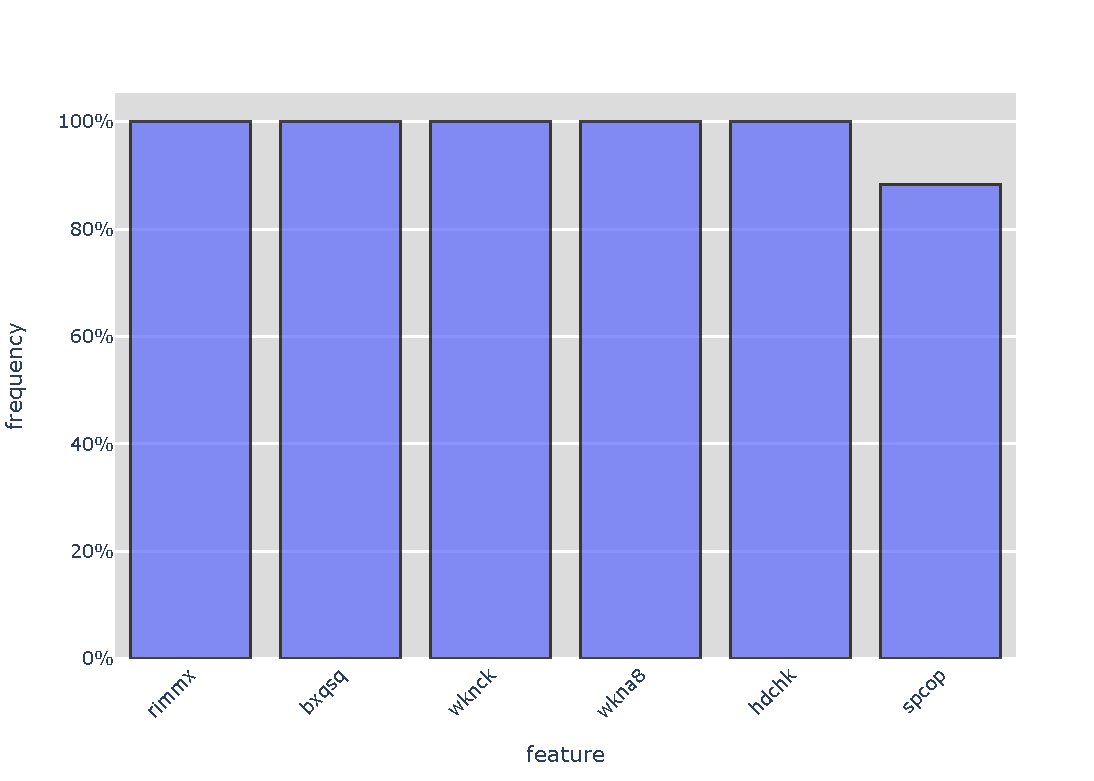
\includegraphics[width=0.8\columnwidth]{figures/chess/featureHistogram.pdf}
    \caption{Histogram of the important features from the `chess' data set.}\label{fig:histChessF}
\end{figure}
\begin{figure}[H]
    \centering
    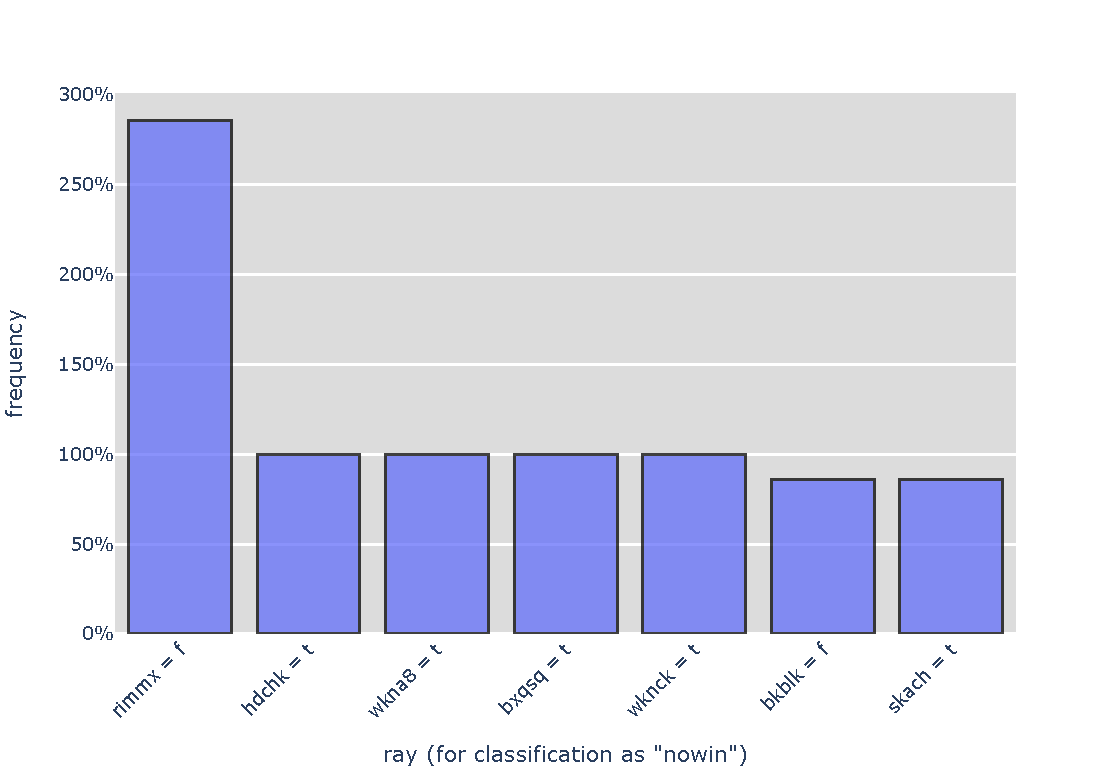
\includegraphics[width=0.8\columnwidth]{figures/chess/raysClass0Histogram.pdf}
    \caption{Histogram of the important class 0 base classifiers from the `chess' data set.}\label{fig:histChessR0}
\end{figure}
\begin{figure}[H]
    \centering
    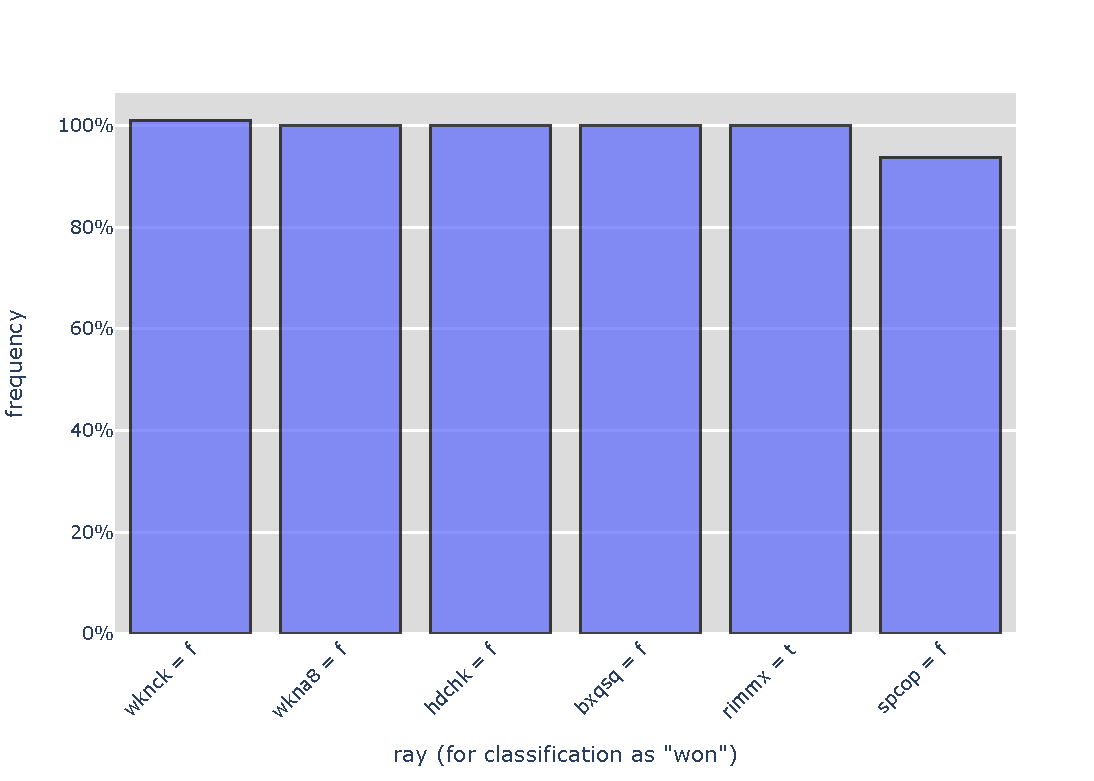
\includegraphics[width=0.9\columnwidth]{figures/chess/raysClass1Histogram.pdf}
    \caption{Histogram of the important class 1 base classifiers from the `chess' data set.}\label{fig:histChessR1}
\end{figure}

\begin{figure}[H]
    \centering
    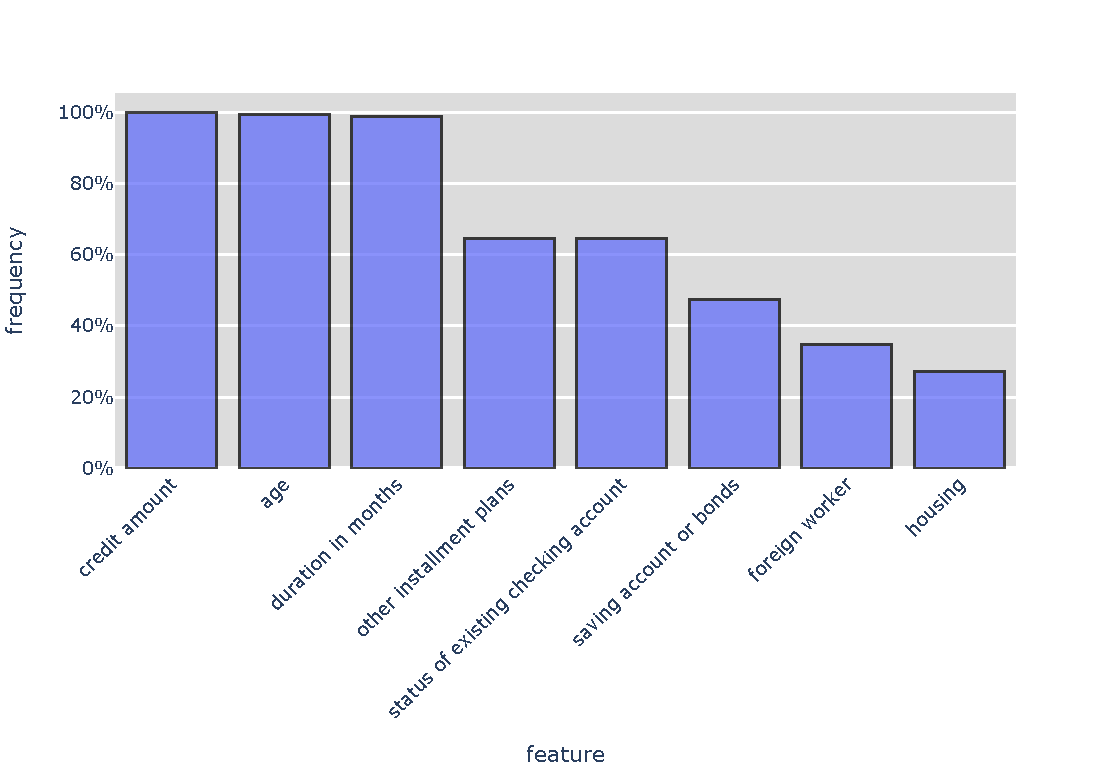
\includegraphics[width=0.9\columnwidth]{figures/german/featureHistogram.pdf}
    \caption{Histogram of the important features from the `german' data set.}\label{fig:histGermanF}
\end{figure}
\begin{figure}[H]
    \centering
    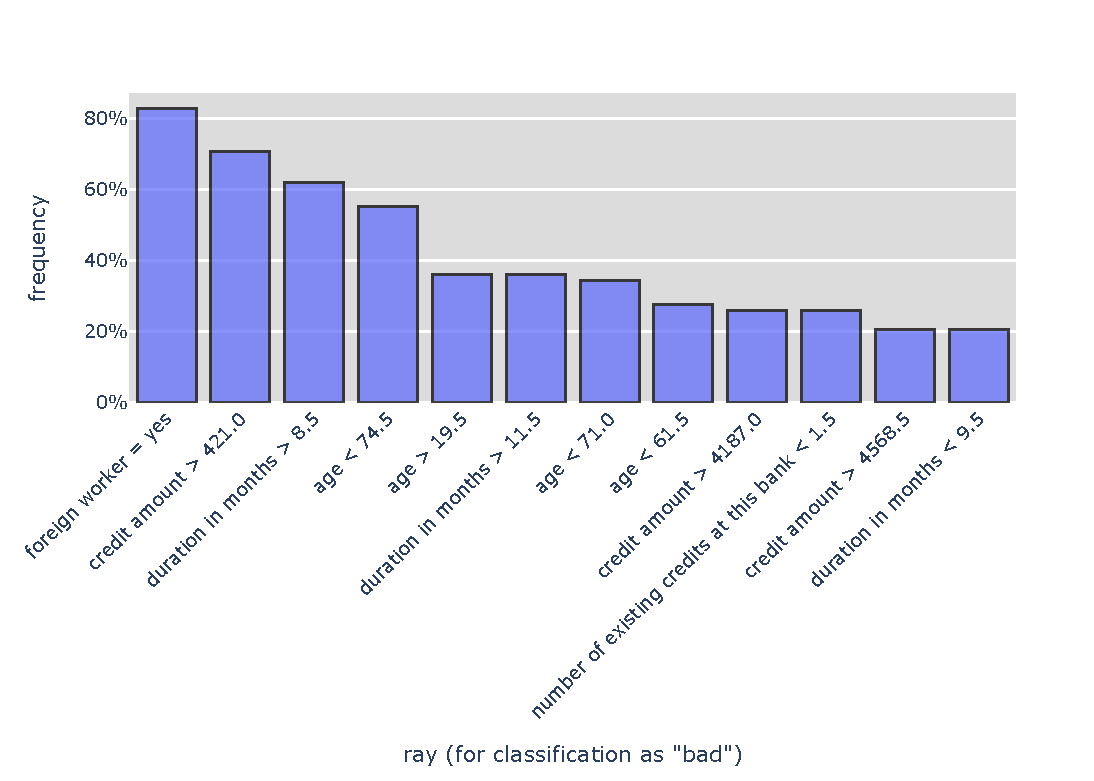
\includegraphics[width=0.9\columnwidth]{figures/german/raysClass0Histogram.pdf}
    \caption{Histogram of the important class 0 base classifiers from the `german' data set.}\label{fig:histGermanR0}
\end{figure}
\begin{figure}[H]
    \centering
    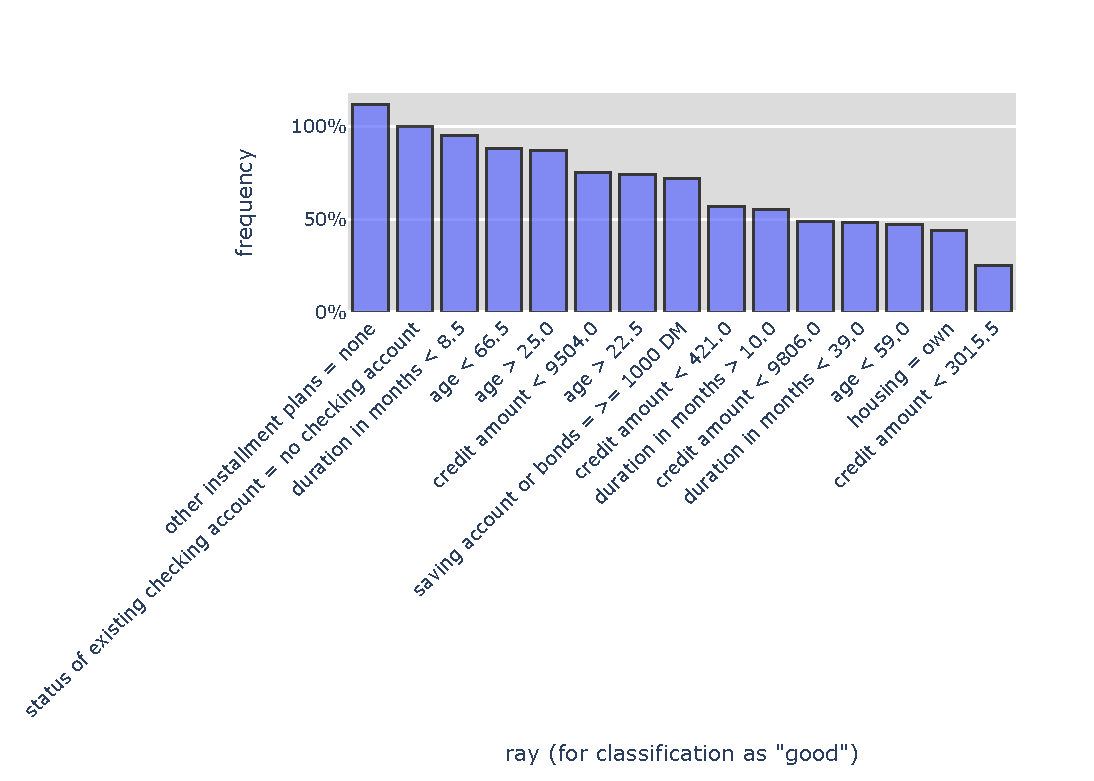
\includegraphics[width=0.9\columnwidth]{figures/german/raysClass1Histogram.pdf}
    \caption{Histogram of the important class 1 base classifiers from the `german' data set.}\label{fig:histGermanR1}
\end{figure}

\begin{figure}[H]
    \centering
    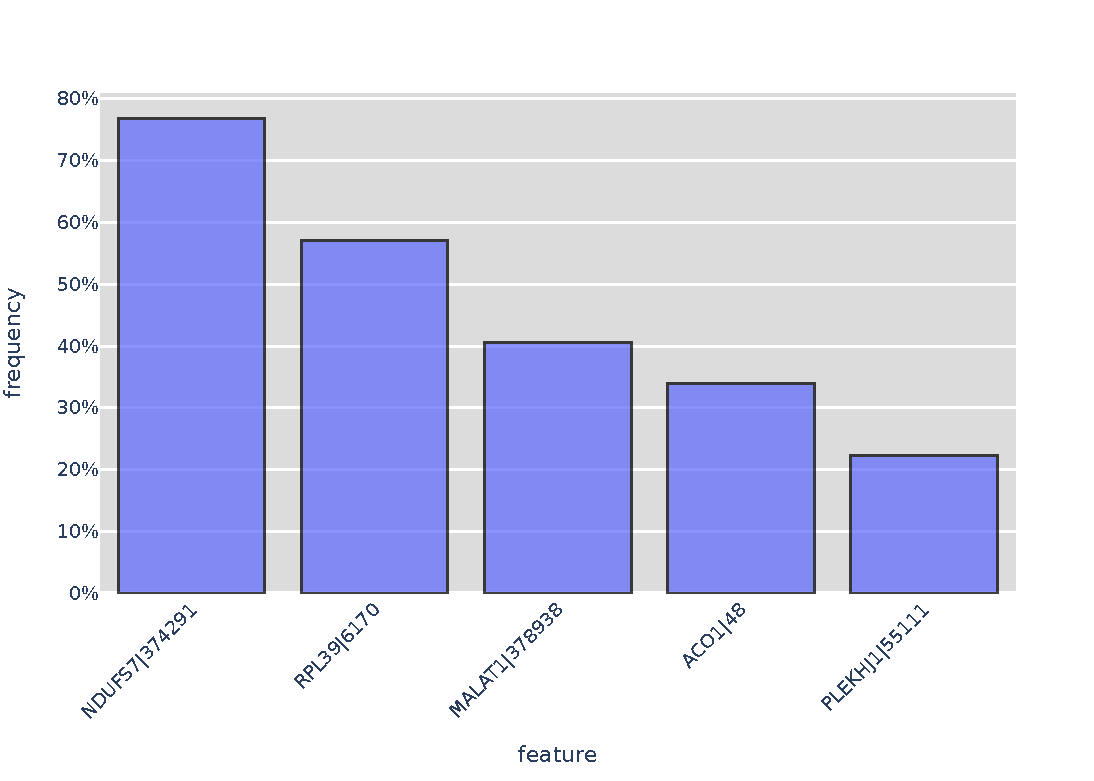
\includegraphics[width=0.9\columnwidth]{figures/genes/featureHistogram_TCGA_KICH_vs_KIRC.pdf}
    \caption{Histogram of the important features from the `KICH\_vs\_KIRC' data set.}\label{fig:histKICHvsKIRC}
\end{figure}
\begin{figure}[H]
    \centering
    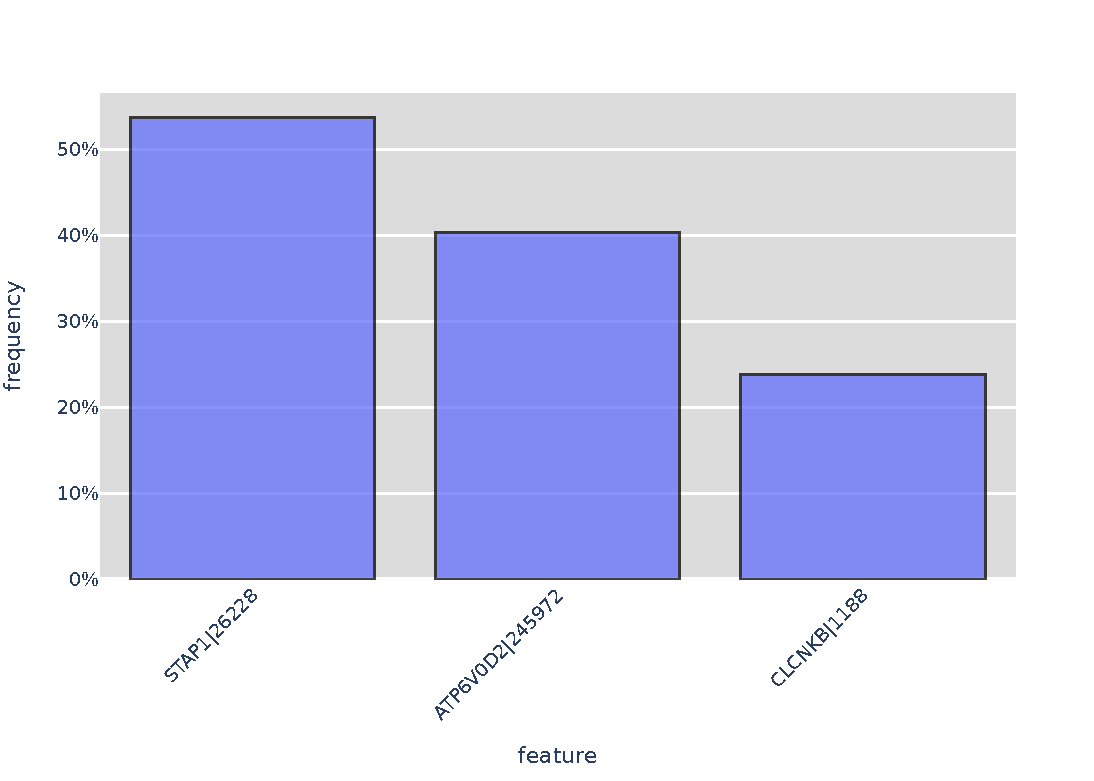
\includegraphics[width=0.9\columnwidth]{figures/genes/featureHistogram_TCGA_KICH_vs_KIRP.pdf}
    \caption{Histogram of the important features from the `KICH\_vs\_KIRP' data set.}\label{fig:histKICHvsKIRP}
\end{figure}
\begin{figure}[H]
    \centering
    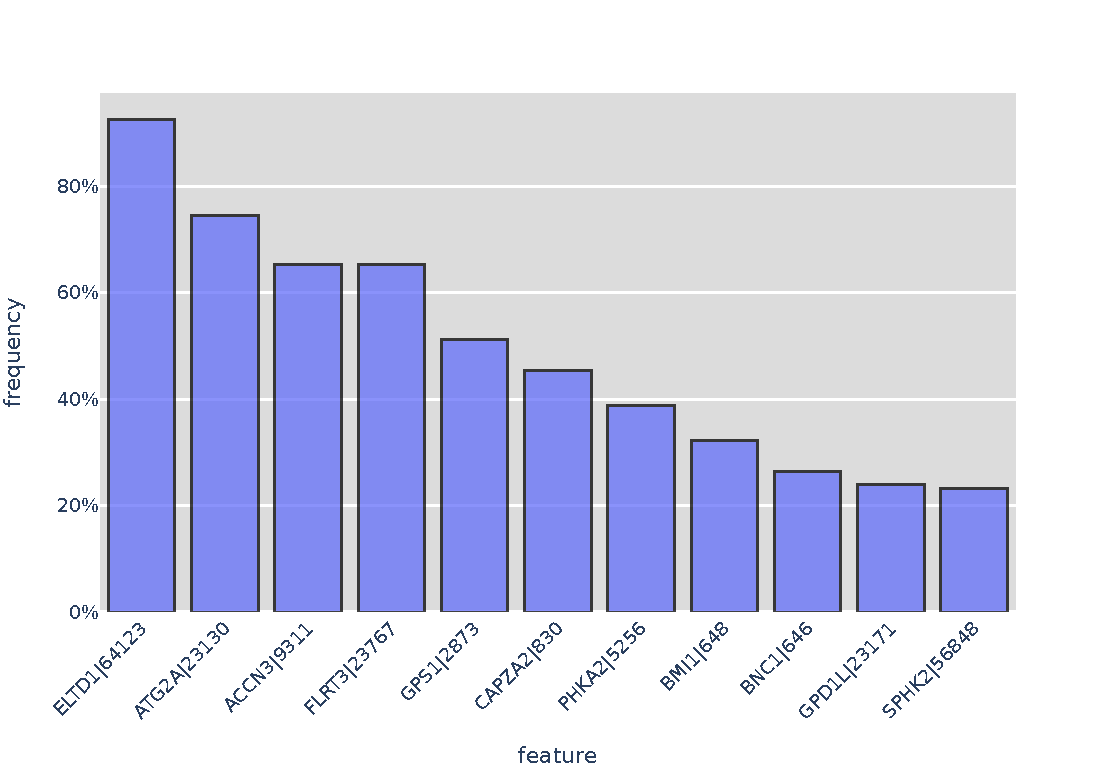
\includegraphics[width=0.9\columnwidth]{figures/genes/featureHistogram_TCGA_KIRP_vs_KIRC.pdf}
    \caption{Histogram of the important features from the `KIRP\_vs\_KIRC' data set.}\label{fig:histKIRPvsKIRC}
\end{figure}
\begin{figure}[H]
    \centering
    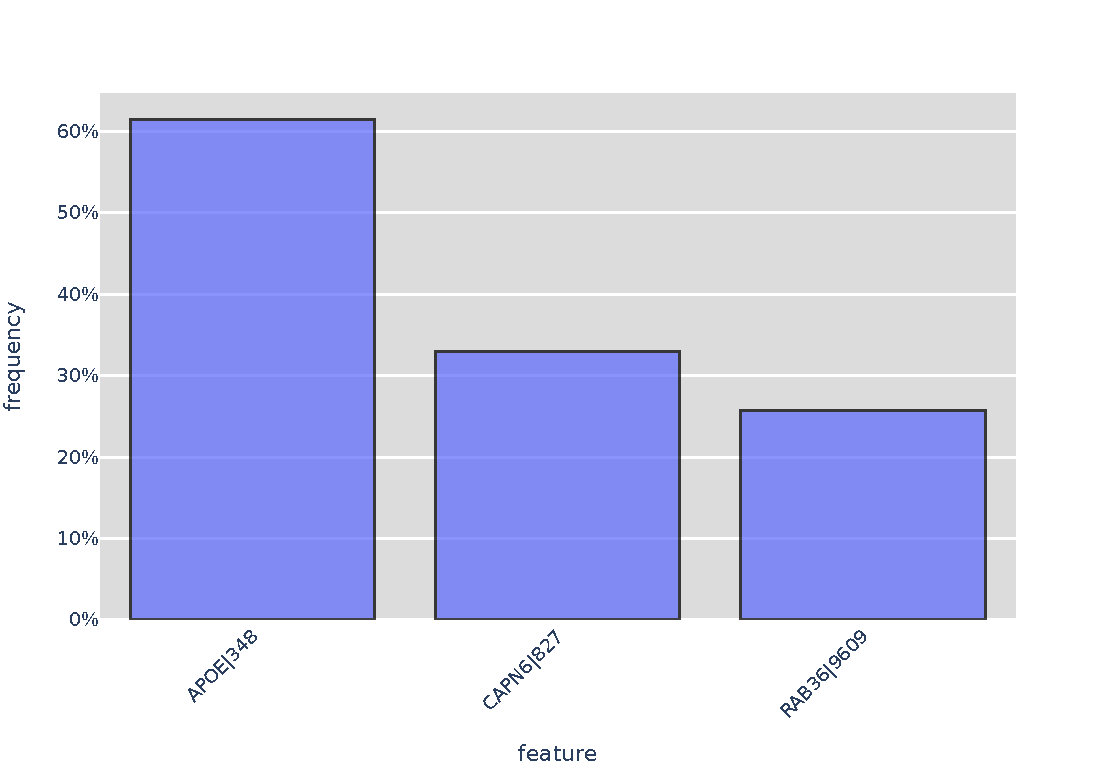
\includegraphics[width=0.9\columnwidth]{figures/genes/featureHistogram_TCGA_CHOL_vs_LIHC.pdf}
    \caption{Histogram of the important features from the `CHOL\_vs\_LIHC' data set.}\label{fig:histCHOLvsLIHC}
\end{figure}
\begin{figure}[H]
    \centering
    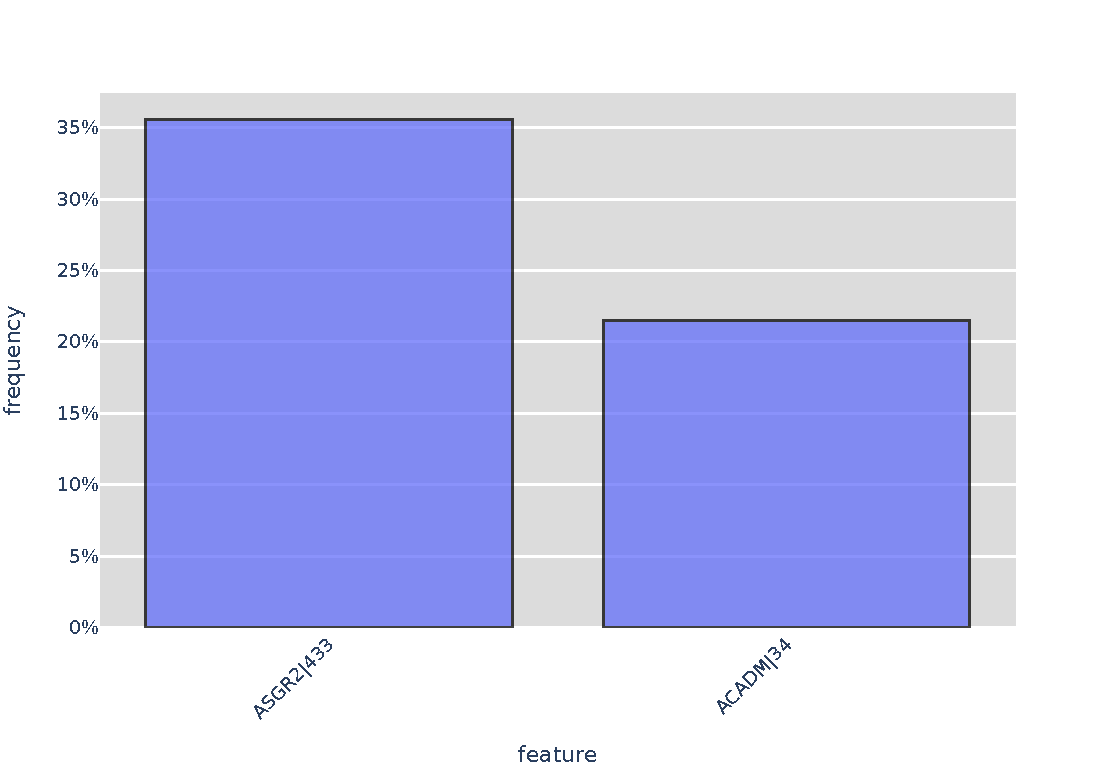
\includegraphics[width=0.9\columnwidth]{figures/genes/featureHistogram_TCGA_CHOL_vs_PAAD.pdf}
    \caption{Histogram of the important features from the `CHOL\_vs\_PAAD' data set.}\label{fig:histCHOLvsPAAD}
\end{figure}
\begin{figure}[H]
    \centering
    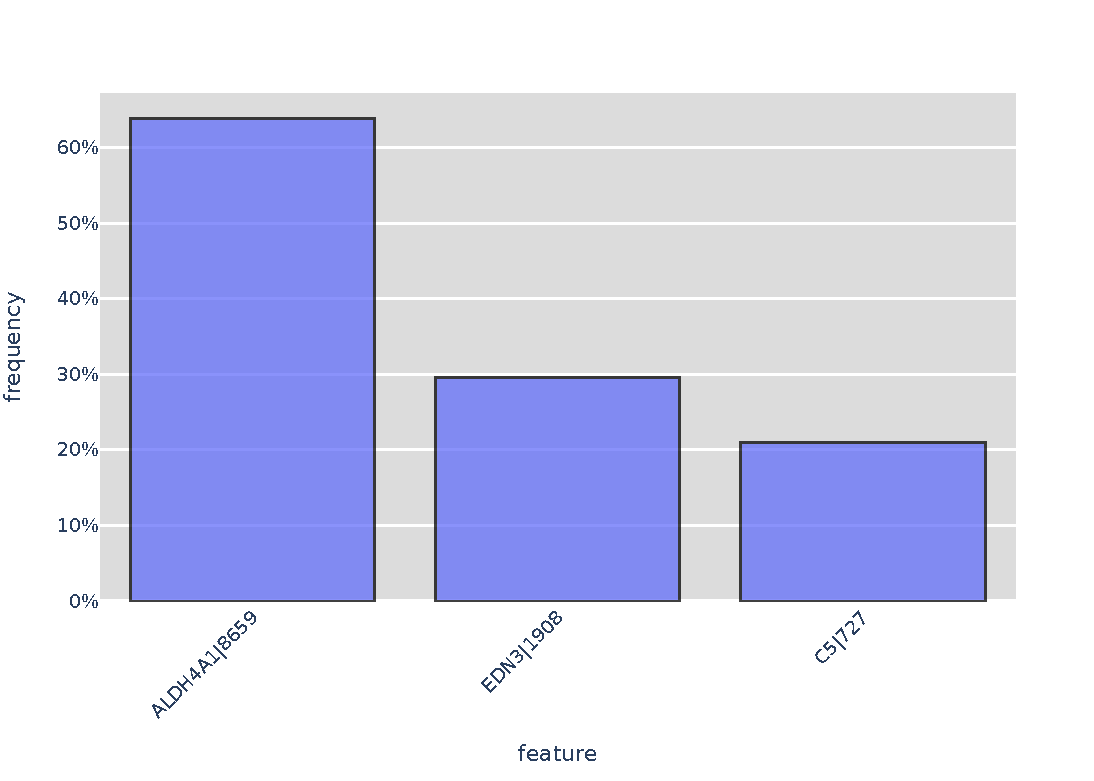
\includegraphics[width=0.9\columnwidth]{figures/genes/featureHistogram_TCGA_LIHC_vs_PAAD.pdf}
    \caption{Histogram of the important features from the `LIHC\_vs\_PAAD' data set.}\label{fig:histLIHCvsPAAD}
\end{figure}
\begin{figure}[H]
    \centering
    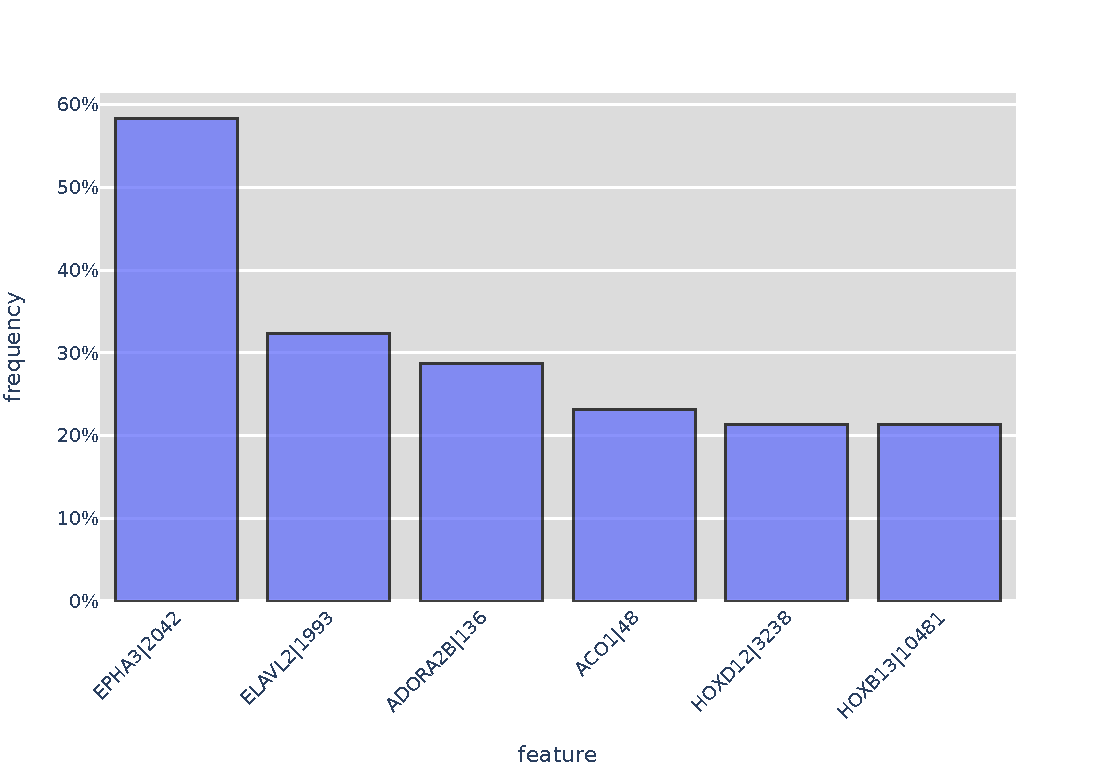
\includegraphics[width=0.9\columnwidth]{figures/genes/featureHistogram_TCGA_COAD_vs_READ.pdf}
    \caption{Histogram of the important features from the `COAD\_vs\_READ' data set.}\label{fig:histCOADvsREAD}
\end{figure}

\clearpage
%%%%%%%%%%%%%%%%%%%%%%%%%%%%%%%%%%%%%%%%%%%%%%%%%%%%%%%%%%%%%%%%%%%%%%%%%%%%%%%%%%%%%%%%%%%%
\section{Julia Source Code}

Listing of all Julia algorithms used in the \autoref{ch:julia} to \autoref{ch:evaluation}.

% chapter 3
\jlinputlisting[label={julia:calcScore},caption={Algorithm calculating a feature's usefulness score.}]{source_code/calc_score.jl}
\jlinputlisting[label={julia:buildConj},caption={Algorithm constructing a conjunction out of multiple optimal base classifiers.}]{source_code/build_conjunction.jl}
\jlinputlisting[label={julia:toString},caption={Algorithm to convert a base classifier, conjunction or disjunction to string using multiple dispatch and recursiveness.}]{source_code/to_string.jl}
\jlinputlisting[label={julia:boolLabels},caption={Algorithm updating a data frame by replacing the labels (usually Strings) by the Boolean classes `true' and `false'. Returning the set of original labels.}]{source_code/bool_labels.jl}
\jlinputlisting[label={julia:findBaseClassifier},caption={Algorithm comparing the return values of \texttt{inspect\_single\_feature} to find the optimum base classifier.}]{source_code/find_ray.jl}

% chapter 4
\jlinputlisting[label={julia:buildDnf},caption={Algorithm constructing a disjunction out of multiple optimal conjunctions.}]{source_code/build_dnf.jl}
\jlinputlisting[label={julia:classify},caption={Algorithm predicting the label of a sample based on a classification rule.}]{source_code/classify.jl}
\jlinputlisting[label={julia:tiesCollect1},caption={Expanding the \texttt{inspect\_single\_feature (NominalFeature)} and \texttt{find\_border} algorithm to collect ties.}]{source_code/ties/collect1.jl}
\jlinputlisting[label={julia:tiesCollect2},caption={Expanding the \texttt{inspect\_single\_feature (NumericalFeature)} algorithm to collect ties.}]{source_code/ties/collect2.jl}
\jlinputlisting[label={julia:tiesCollect3},caption={Expanding the \texttt{find\_base\_classifier} algorithm to collect ties.}]{source_code/ties/collect3.jl}
\jlinputlisting[label={julia:buildConjTies},caption={Expansion of the \texttt{build\_conjunction} algorithm that uses and collects ties.}]{source_code/ties/build_conj.jl}
\jlinputlisting[label={julia:buildDnfTies},caption={Expanding the \texttt{build\_dnf} algorithm to use ties.}]{source_code/ties/build_dnf.jl}

% chapter 5
\jlinputlisting[label={julia:loadCsv},caption={Algorithm parsing fixed width strings from a CSV file into regular strings.}]{source_code/load_csv.jl}
\jlinputlisting[label={julia:inspectNumerical},caption={Algorithm identifying the optimal ray on a specific numerical feature.}]{source_code/inspect_single_feature_num.jl}
\jlinputlisting[label={julia:findBorder},caption={Algorithm identifying the optimal ray for a specific operator on a specific numerical feature.}]{source_code/find_border.jl}
\jlinputlisting[label={julia:preventRecorr},caption={Algorithm preventing the SCM to choose rays that would override previously selected rays.}]{source_code/prevent_recorr.jl}
\jlinputlisting[label={julia:thresholdInbetween},caption={Algorithmic extension to maximize a ray's margins.}]{source_code/threshold_inbetween.jl}
\jlinputlisting[label={julia:inspectNominal},caption={Algorithm identifying the optimal base classifier on a specific nominal feature.}]{source_code/inspect_single_feature_nom.jl}

% chapter 6
\jlinputlisting[label={julia:cv},caption={Most important parts of the \(m \times n\) cross-validation algorithm.}]{source_code/cross_validation.jl}
\jlinputlisting[label={julia:paretoFront},caption={Algorithm computing all models on the first pareto front.}]{source_code/pareto_front.jl}
\jlinputlisting[label={julia:loadRData},caption={Algorithm to load the modified TCGA data sets from~\cite{lausser20}.}]{source_code/load_rdata.jl}